
\begin{document}
Принципиальная схема:
\begin{center}
        \begin{figure}[h!]
                \center{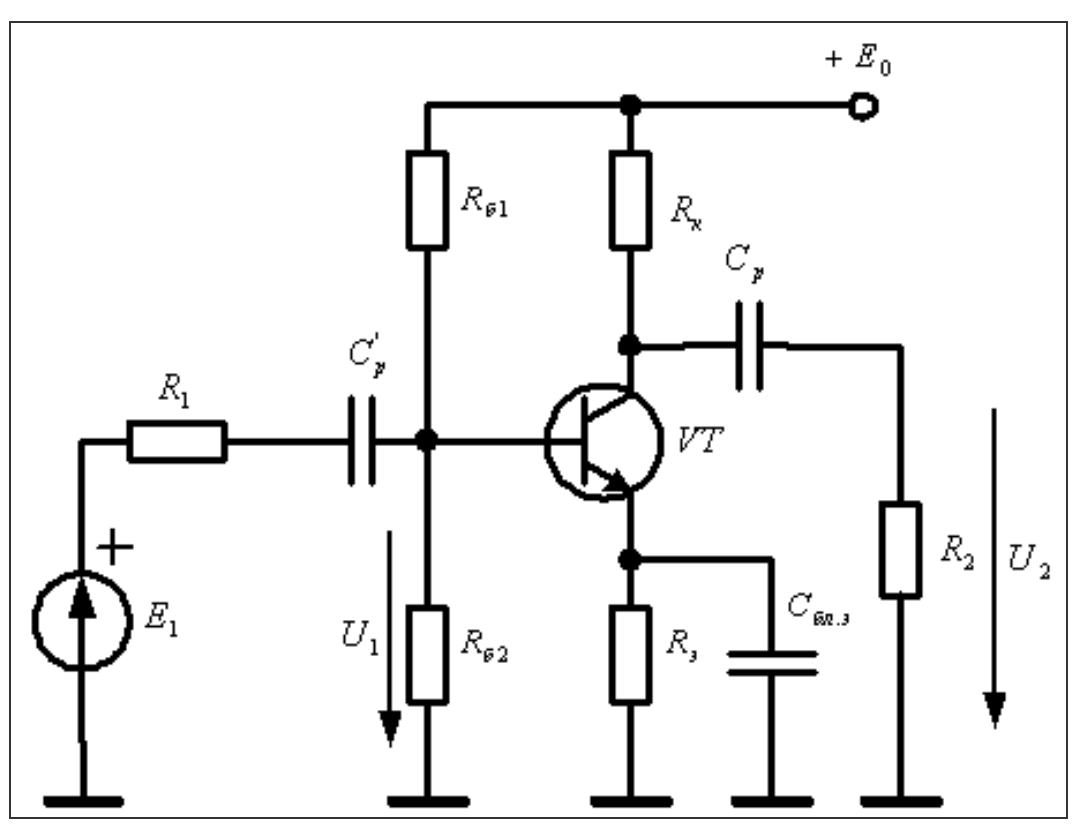
\includegraphics[scale=0.2]{oe.png}}
                \caption{Чем принципиально отличаеются усилительные каскады на БТ и УПТ?}
        \end{figure}
\end{center}
Каскады на БТ и УПТ имеют одинаковое назначение -- усиление сигнала. Но принцип их управления и действия по некоторым параметрам отличается.

//ЗДесь рассматриваются все шесть каскадов попарно+дополнительные выводы , указанные ниже  //В КАЖДОМ ПУНКТЕ МОЖНО ВСТАВИТЬ ССЫЛКИ НА НИХ 

1) Каскад ОЭ == ОИ
оба инвертируют фазу и хорошо усиливают как напряжение,так и ток.
Входное сопротивление ОИ >> входного сопротивления каскада ОЭ.
Входное сопротивление ОЭ достигает десятки ОМ, в то время как входное ОИ до 3МОм, так как там используется обратно смещенный p-n переход.

Но выходное сопротивление ОЭ больше его же входного сопротивления, следовательно у него согласующие свойства намного хуже, чем у ОИ.


2) каскад ОБ == ОЗ
Коэффициенты усиления по напряжению у них не очень хорошие+малые входные  большие выходные сопротивления => плохие согласующие свойства

P.s. $R_\textit{вхтроз} = 1/S$ - мало

3) Каскады ОК == ОС
Оба каскада обладают большим входным сопротивлением, причем $R_\textit{вхтрос} ~ 1$ МОм, и оба каскада обладают очень маленьким выходным сопротивлением, поэтому у них очень лучшие согласующие свойства среди всех типов каскадов, но усиление у них хуже, чем у ОЭ(ОИ)

Однако основным и наиболее важным отличием между каскадами на УПТ и БТ является то, что каскады на ПТ управляются напряжением на ЗИ , а на БТ  - током. Следовательно, мощность, которая требуется для управления ПТ, будет меньше, чем для БТ: управление электрическим полем гарантирует отсутствие входных токов => больше входное сопротивление, высокая нагрузочная способность ПТ в
 ключевом режиме.

В БТ В - коэффициент, характеризующий усиление по току, $B = I_K/I_b$ -- во сколько раз коллекторный ток превышет базовый.
$\alpha = I_K/I_E$.

//тут должна быт система из двух уравнений
(1)$I_K = \alphaI_e+I\textit{ут}+I\textit{т}$
(2)$I_e = I_K+I_b$
//
=>$I_K = \alpha(I_b+I_k)+I\textit{k0}= \alpha/(\alpha+1)I_b+1\(1-\alpha)I_\textit{k0}=bI_b+(1+B)I\textit{k0}$
=> Ik ~ BIb => любое изменение тока Б порождает изменение тока К.
ПТ - управляется Uзи (электрическое поле) осуществляющее изменение поперечного сечения проводящего канала => изменяется ток транзситора (С-И):


КАРТИНКА upt.png
$I_c = b[(U_\textit{зи} - U_\textit{пор})_\textit{си}-1/2(U_\textit{cи})^2]$
$I_c =f(U_\textit{зи}, U_\textit{cи})$

$S = dI_\textit{cи}/(dU_\textit{pи}) $ при $U_\textit{cи}=const$

!!Дополнительно
В БТ есть эффект модуляции базы, возникающий засчет расширения (сужения ) КП транзистора, при этом есть вероятность смыкания КП и ЭП.
Рассмотрим УПТ

КАРТИНКА upt1.png
здесь Rси отражает эффект модуляции длины канала.


